\documentclass[12pt]{article}

\usepackage{amsmath}
\usepackage{graphicx}

\begin{document}

\section{Dynamical System}

The following ODEs govern calcium ($c$) dynamics

\begin{align}
\frac{dc}{dt} &= J_{IP3R} + J_{ERleak} - J_{SERCA} \quad + \delta [J_{ECSadd} - J_{PMCA} + J_{SOC}] \\
\frac{dc_{tot}}{dt} &= \delta [J_{ECSadd} - J_{PMCA} + J_{SOC}] \\
\frac{dh}{dt} &= \frac{h_{\infty} - h}{\tau_h}
\end{align}

where the equations related to $h$ are
\begin{align}
\tau_h &= \frac{1}{a_2(Q_2 + c)} \\ 
\quad h_{\infty} &= \frac{Q_2}{Q_2 + c} \\
Q_2 &= d_2\biggr(\frac{p+d_1}{p+d_3} \biggr)
\end{align}

The various fluxes $J$ are given each by
\begin{align}
J_{IP3R} &= v_{IP3R} m_{\infty}^3 n_{\infty}^3 h^3 (c_{ER} - c) \\
m_{\infty} &= \frac{p}{p+d_1}, \quad n_{\infty} = \frac{c}{c+d_5} \\
J_{SERCA} &= v_{SERCA} \frac{c^{1.75}}{c^{1.75} + k_{SERCA}^{1.75}} \\ 
J_{PMCA} &= v_{PMCA} \frac{c^2}{c^2 + k_{PMCA}^2} \\
J_{SOC} &= v_{SOC} \frac{k_{SOC}^2}{k_{SOC}^2 + c_{ER}^2} \\
J_{ERleak} &= v_{ERleak}(c_{ER} - c)\\
J_{ECSadd} &= v_{in} - k_{out}c
\end{align}

and in equations (1), (2), $\delta$ is a scaling size parameter. The other dynamic variable of interest is IP3 ($p$), which has ODEs

\begin{align}
IP3_{production} &= v_{\beta}G^* + v_{\delta} \frac{k_{\delta}}{1+p} \frac{c^2}{c^2 + k_{PLC\delta}^2} \\
IP3_{degradation} &= v_{3k} \frac{c^4}{c^4 + k_d^4} \frac{p}{p+k_3} + r_{5p}p \\
\frac{dp}{dt} &= IP3_{production} - IP3_{degradation}
\end{align}

$G^*$ is the strength of external stimulation to the system and our bifurcation parameter. Importantly in equations (14) and (15), $v_{\delta}$ is the strength of positive $c \rightarrow p$ feedback, and $v_{3k}$ is the strength of negative $c \rightarrow p$ feedback. If $v_{\delta}=0$ or $v_{3k}=0$ , we say that there is no positive or no negative feedback respectively.


\section{Observation of Delay}

We apply a long pulse of $G^*$ to the system, and are interested in looking at how long it takes for the system to reach a stable oscillation cycle in the $c$ variable. For smaller stimulation strength $G^*=0.07$), this is quick to occur after the initial spike in $c$. For larger stimulation, there is a progressively longer delay when there is negative $c \rightarrow p$ feedback in the system.

\begin{figure}[h!]
	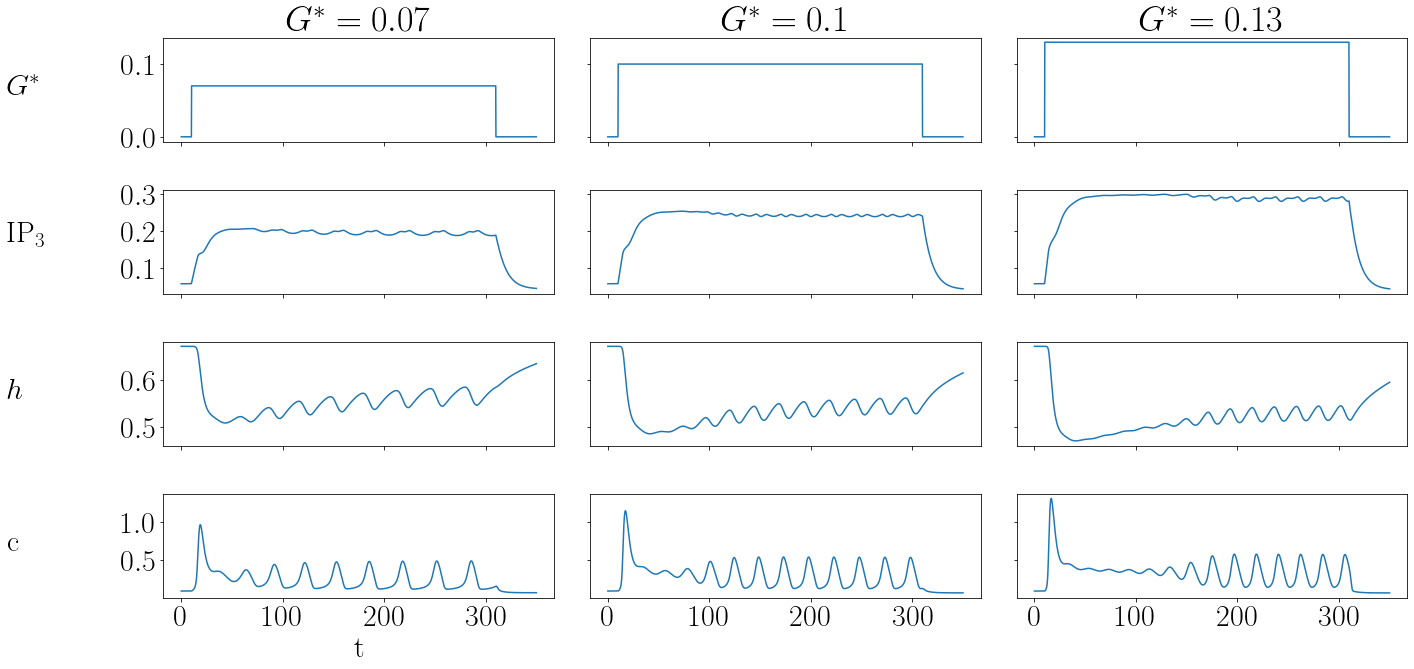
\includegraphics[width=1\linewidth]{varying_Gstar_oscillation_delays.png}		
\end{figure}

\subsection{Variation of Negative Feedback Strength}

Note that increases to $c \rightarrow p$ negative feedback exacerbate the oscillation delays. Positive feedback appears to have no effect. (For all other figures, $v_{3k} = 0.1$)

\begin{figure}[h!]
	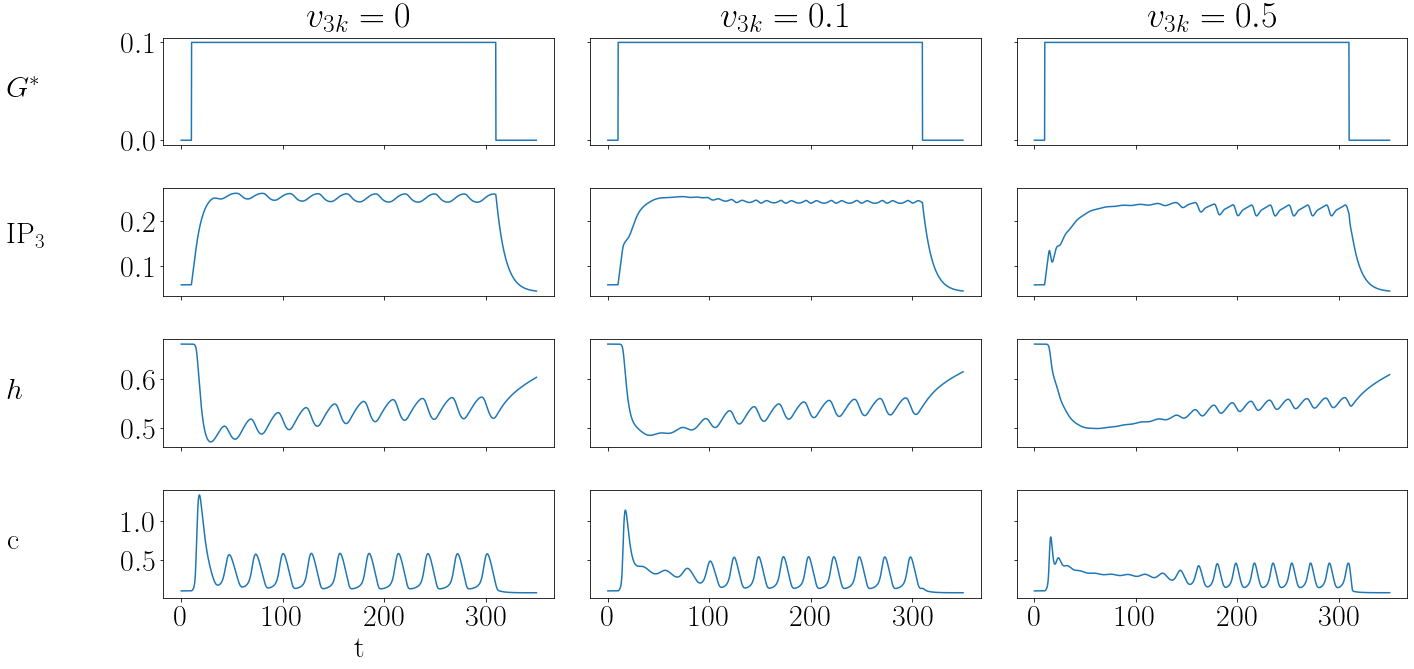
\includegraphics[width=1\linewidth]{varying_v3k.png}		
\end{figure}

\section{Bifurcations}

When $p$ is used as a control parameter we can produce the following bifurcation diagram in $p$, $c$ space:

\begin{figure}[h!]
	\centering
	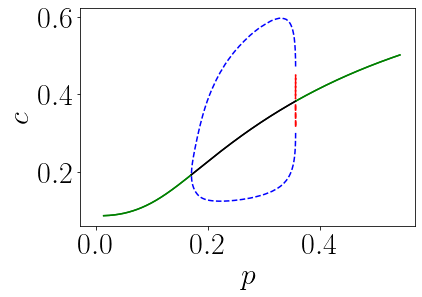
\includegraphics[width=0.5\linewidth]{ip3_ca_bifurcation.png}		
\end{figure}

We plot the $p$-$c$ trajectories from the previous section against this bifurcation diagram (noting that trajectories do not conform exactly to the bifurcation diagram since $p$ is now a variable)

\begin{figure}[h!]
	\centering
	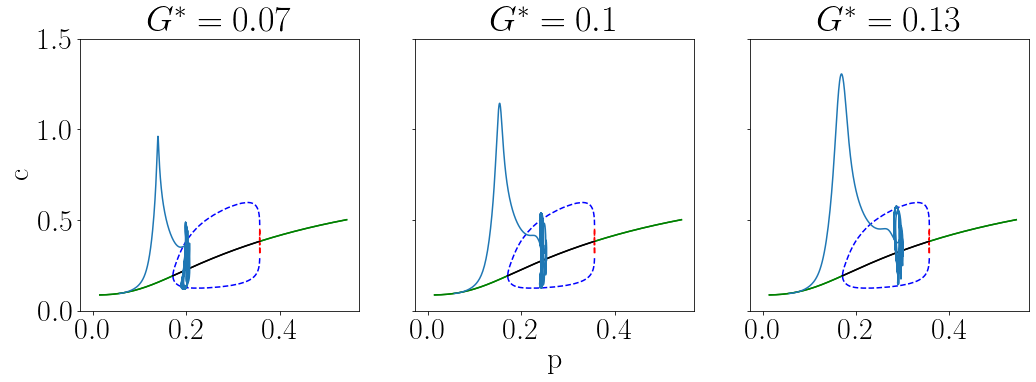
\includegraphics[width=1\linewidth]{trajectories_on_bifurcation_p_c.png}		
\end{figure}

A movie of the above diagram is available with the file name ``trajectories\_on\_bifurcation\_p\_c.mp4''. 

\subsection{G* Bifurcations}

Looking at bifurcations in the full system (including $p$ as a variable) with $G^*$ as the control parameter, we produce the following bifurcation plots, where positive and negative $c \rightarrow p$ feedback is either turned on or off.

\begin{figure}[h!]
	\centering
	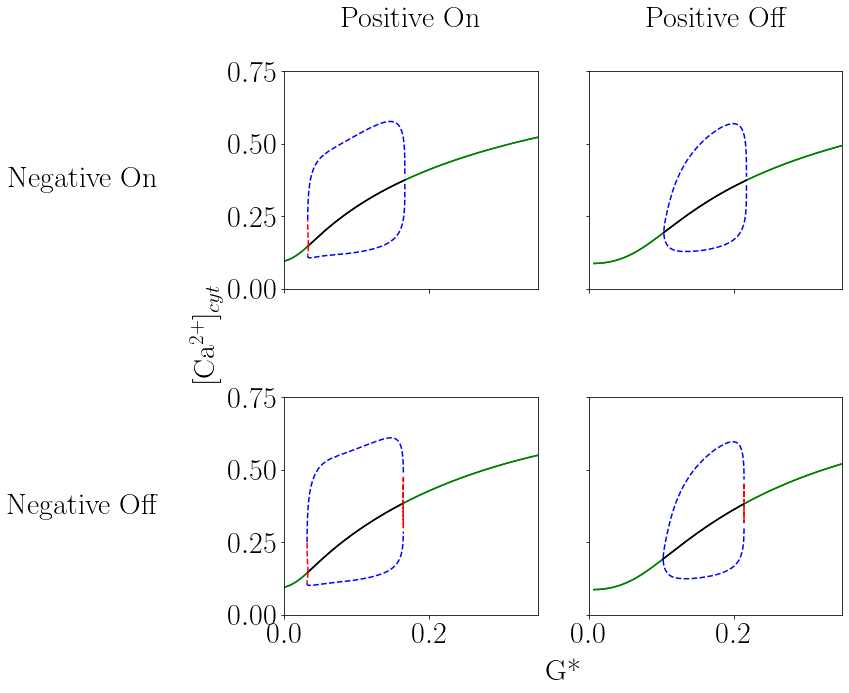
\includegraphics[width=1\linewidth]{positive_negative_bifurcations.png}		
\end{figure}

\end{document}

